\documentclass[12pt]{article}
\usepackage{geometry}
\geometry{a4paper}
\usepackage[utf8]{inputenc}
\usepackage{amsmath,amssymb}
\usepackage{hyperref} % verlinkungen
\usepackage{textcomp}
\usepackage{flafter}
\usepackage{booktabs}
\usepackage{array}
\usepackage{paralist}
\usepackage{dsfont} \usepackage{color}
\usepackage{bbold}
\usepackage{float}
\usepackage[font=scriptsize,labelfont=bf]{caption}
%\usepackage[font=footnotesize,labelfont=bf]{caption}
%\usepackage{subcaption}
\usepackage{fancyhdr}
\setlength{\headheight}{15.2pt}
\pagestyle{fancy}
\usepackage{listings} 
\usepackage{pict2e}
\usepackage{xfrac}
\usepackage[english]{babel}
\usepackage{mathtools}
\usepackage{graphicx}



%%%%%%%%         EIGENEBEFEHLE  %%%%%%%%%
\newcommand{\ddt}{\frac{\partial}{\partial{t}}}
\newcommand{\dnach}[1]{\frac{\partial}{\partial{#1}}}
\newcommand{\ddnach}[2]{\frac{\partial{#1}}{\partial{#2}}}
\newcommand{\dddnach}[3]{\frac{\partial^2{#1}}{\partial{#2} \partial{#3}}}
\newcommand{\dznach}[2]{\frac{\partial^2{#1}}{\partial{#2}^2}}
\newcommand{\vnabla}{\vec{\nabla}}
\newcommand{\evec}[1]{\mathbf{\hat{#1}}}
\newcommand{\bra}[1]{\langle{#1}|}
\newcommand{\ket}[1]{|{#1}\rangle}
\newcommand{\bracket}[2]{\langle{#1}|{#2}\rangle}
\newcommand{\up}{\uparrow}
\newcommand{\down}{\downarrow}
\newcommand{\updown}{\uparrow\downarrow}
\newcommand{\downup}{\downarrow\uparrow}
\newcommand{\upup}{\uparrow\uparrow}
\newcommand{\downdown}{\downarrow\downarrow}
\newcommand{\sandwich}[2]{\bra{#1} #2 \ket{#1}}
\newcommand{\fsqrt}[2]{\sqrt{\frac{#1}{#2}}}

\definecolor{mygreen}{rgb}{0,0.6,0}
\definecolor{mygray}{rgb}{0.5,0.5,0.5}
\definecolor{mymauve}{rgb}{0.58,0,0.82}

\lstset{%
  backgroundcolor=\color{white},   % choose the background color; you must add \usepackage{color} or \usepackage{xcolor}
  basicstyle=\footnotesize,        % the size of the fonts that are used for the code
  breakatwhitespace=false,         % sets if automatic breaks should only happen at whitespace
  breaklines=true,                 % sets automatic line breaking
  captionpos=b,                    % sets the caption-position to bottom
  commentstyle=\color{mygreen},    % comment style
  %deletekeywords={...},            % if you want to delete keywords from the given language
  %escapeinside={\%*}{*)},          % if you want to add LaTeX within your code
  extendedchars=true,              % lets you use non-ASCII characters; for 8-bits encodings only, does not work with UTF-8
  frame=single,                    % adds a frame around the code
  keepspaces=true,                 % keeps spaces in text, useful for keeping indentation of code (possibly needs columns=flexible)
  keywordstyle=\color{blue},       % keyword style
  language=C,                 % the language of the code
  %morekeywords={*,...},            % if you want to add more keywords to the set
  numbers=left,                    % where to put the line-numbers; possible values are (none, left, right)
  numbersep=5pt,                   % how far the line-numbers are from the code
  numberstyle=\tiny\color{mygray}, % the style that is used for the line-numbers
  rulecolor=\color{black},         % if not set, the frame-color may be changed on line-breaks within not-black text (e.g. comments (green here))
  showspaces=false,                % show spaces everywhere adding particular underscores; it overrides 'showstringspaces'
  showstringspaces=false,          % underline spaces within strings only
  showtabs=false,                  % show tabs within strings adding particular underscores
  stepnumber=2,                    % the step between two line-numbers. If it's 1, each line will be numbered
  stringstyle=\color{mymauve},     % string literal style
  tabsize=2,                       % sets default tabsize to 2 spaces
  %title=\lstname                   % show the filename of files included with \lstinputlisting; also try caption instead of title
}

\lhead[\ ]{\ }
\chead[\ ]{\ }
\rhead[\ ]{\ }

\lfoot[\ ]{\ }
\cfoot[\ ]{\ }
\rfoot[\ ]{\ }

%%%%%%%%%%%%%%%%%%%%%%%%%%%%%%%%%%%%%%%%%%%%

\begin{document}
\title{Temperature Measurements in Optical Tweezer Experiments}
\author{Mathias H\"old, BSc.}
\date{2016}
\maketitle
\thispagestyle{empty}
\newpage
\section{Introduction}
%something about computer science in general, optical tweezers and the need to study the
%systems on computers yada yada





\newpage
\section{Motivation}
%introduction of the experiment, the problem and the idea
\section{The experiment}
The starting point of this thesis is an experiment conducted by Gieseler et al \cite{Gieseler2014}. It is an optical tweezer experiment, where the
motion of a glass nanoparticle in a laser trap was used to investigate the fluctuation theorem\cite{Crooks1999}.
\subsection{Experimental setup}
In the experiment, a silica nano particle with a radius of about 75 nm and mass of about $3 \times 10^{-18}$kg is trapped in a laser beam within a
vacuum chamber. The trapping of the silica nano particle (which will be referred to as \textit{glass particle}) is achieved by a gradient force of the
laser beam acting on the particle. The experimental setup is depicted in fig. \ref{fig:setup}.\\
The particle fluctuates within the trap in all three spatial directions. These fluctuations can be approximated
such that they are decoupled, which means that they can be described by a 1-dimensional Langevin equation:
\begin{equation}
    \ddot{x} + \Gamma_0 \dot{x} + \Omega^2_0x = \frac 1 m \left(F_\text{fluct} + F_\text{ext}\right)
\end{equation}
%The experiment is set up as follows: a glass sphere with radius $r \approx 75$ nm and mass $m \approx 3 \times 10^{-18}$ kg is trapped in a laser beam
%in a vacuum chamber. The initial state of the glass particle is prepared by modulation of the laser, such that the oscillation of the glass particle
%is suppressed in every direction. This is done by measuring the oscillation of the particle in every direction (assuming that the oscillation in every
%direction is decoupled) and using this information as feedback for the laser. This experimental setup can be seen in figure \ref{fig:setup}.
\begin{figure}[H]
    \begin{center}
        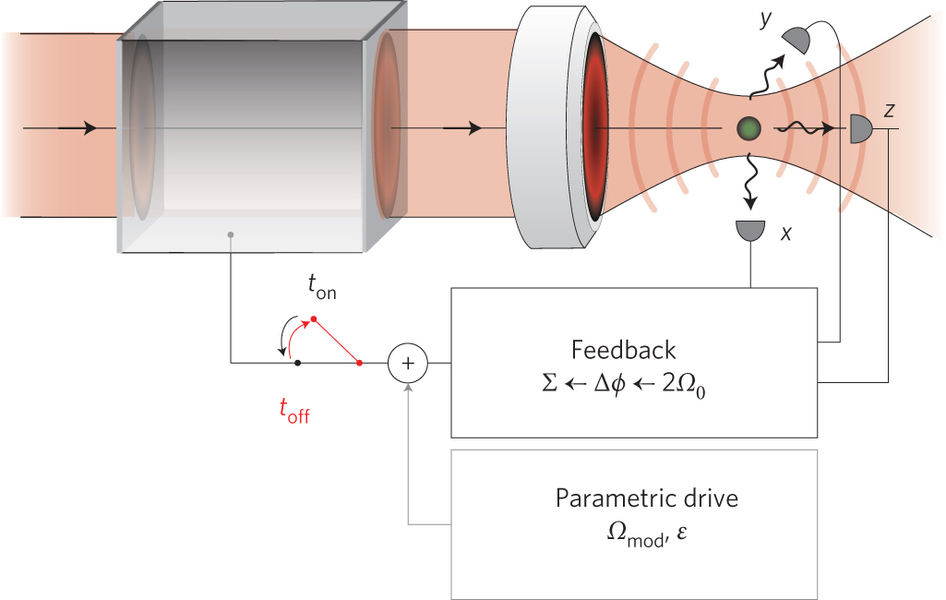
\includegraphics[scale=0.3]{images/experimental_setup.jpg}
        \caption{Experimental setup of the optical tweezer experiment. A silica nano particle is trapped in a laser beam via gradient force in a
        vacuum. The feedback is used to cool down the particle and create a non-equilibrium steady state. In the first part of the experiment, the
    feedback is turned off and the motion of the particle towards an equilibrated state is observed. In the second part of the experiment, the steady state
of the particle is modified by a parametric drive. Both the parametric drive and the feedback are turned off and -- as in the first part -- the
motion of the particle towards an equilibrated state is observerd.}
        \label{fig:setup}
    \end{center}
\end{figure}
On the left hand side we have the friction coefficient $\Gamma_0$ and the angular frequency that describes the fluctuation along the chosen axis. On
the right hand side, there are two forces. The first one is $F_\text{fluct}$, which describes a stochastic force caused by interactions with the gas
in the vacuum chamber. This force is given by
\begin{equation}
    F_\text{fluct} = \sqrt{2m\Gamma_0k_BT_0} \ \xi\left(t\right)
\end{equation}
where $T_0$ is the temperature of the heat bath (i.e. the surrounding gas in the vacuum chamber), $k_B$ is the Boltzmann constant and $\xi(t)$ is
white noise, which obeys the equations $\left\langle\xi(t)\right\rangle= 0$ and $\left\langle\xi(t)\xi(t')\right\rangle= \delta(t-t')$, which means
that it is a random force. The term $\Gamma_0$ appears in the formulat due to the fluctuation-dissipation theorem, which links the damping rate to the
stochastic force.\\
The external force $F_\text{ext}$ is part of the experimental setup, where the frequency of the fluctuation along an axis, $\Omega_0$, is measured and
used to suppress the motion along said axis. This causes a decrease in the particle fluctuations and thus acts as a cooling mechanism for the particle
in the trap. This process creates a non-equilibrium steady state $\rho_{ss}(u,\alpha)$, which is not known analytically. This state is the starting
point of this thesis.\\








\newpage
\section{Simulation}
%simulation techniques and general concept of the simulation itself, used methods and so on 
The problem at hand can be studied on an atomic level with the use of computer simulation. There is a variety of methods for computer simulations
that are widely used, one of which being Molecular Dynamics (MD) simulations. The following section will give a brief overview of the concepts of this
method, which is followed by the application to the simulation of the experiment.

\subsection{Molecular Dynamics}
Molecular Dynamics\cite{Frenkel2001} simulations is a technique for simulating, as the name suggests, the dynamics of a classical many-body system. In this case,
classical means, that the trajectories of the individual particles are calculated using classical mechanics rather then quantum mechanics. For
relatively big atoms/molecules this is a very good approximation, whereas for systems consisting of hydrogen or helium the effects of quantum
mechanics cannot be neglected and other methods (such as ab-initio simulation) has to be used.\\
The dynamics of the system are obtained by solving Newton's equations of motion for every particle. 

\subsection{The Glass Particle}
The glass particle from the experiment will be modeled as a system of particles interacting via a Lennard-Jones pair potential, 
\begin{equation}
    \label{eq:lj}
    U(r) = 4\varepsilon\left[\left(\frac\sigma r\right)^{12} - \left(\frac\sigma r\right)^6\right]
\end{equation}
where $\varepsilon$ is the depth of the potential well (and thus its unit is energy) and $\sigma$ is the distance at which the potential is zero. 
The form of the potential and the relation to the parameters is depicted in Fig. \ref{fig:lj}.
\begin{figure}[h]
    \begin{center}
        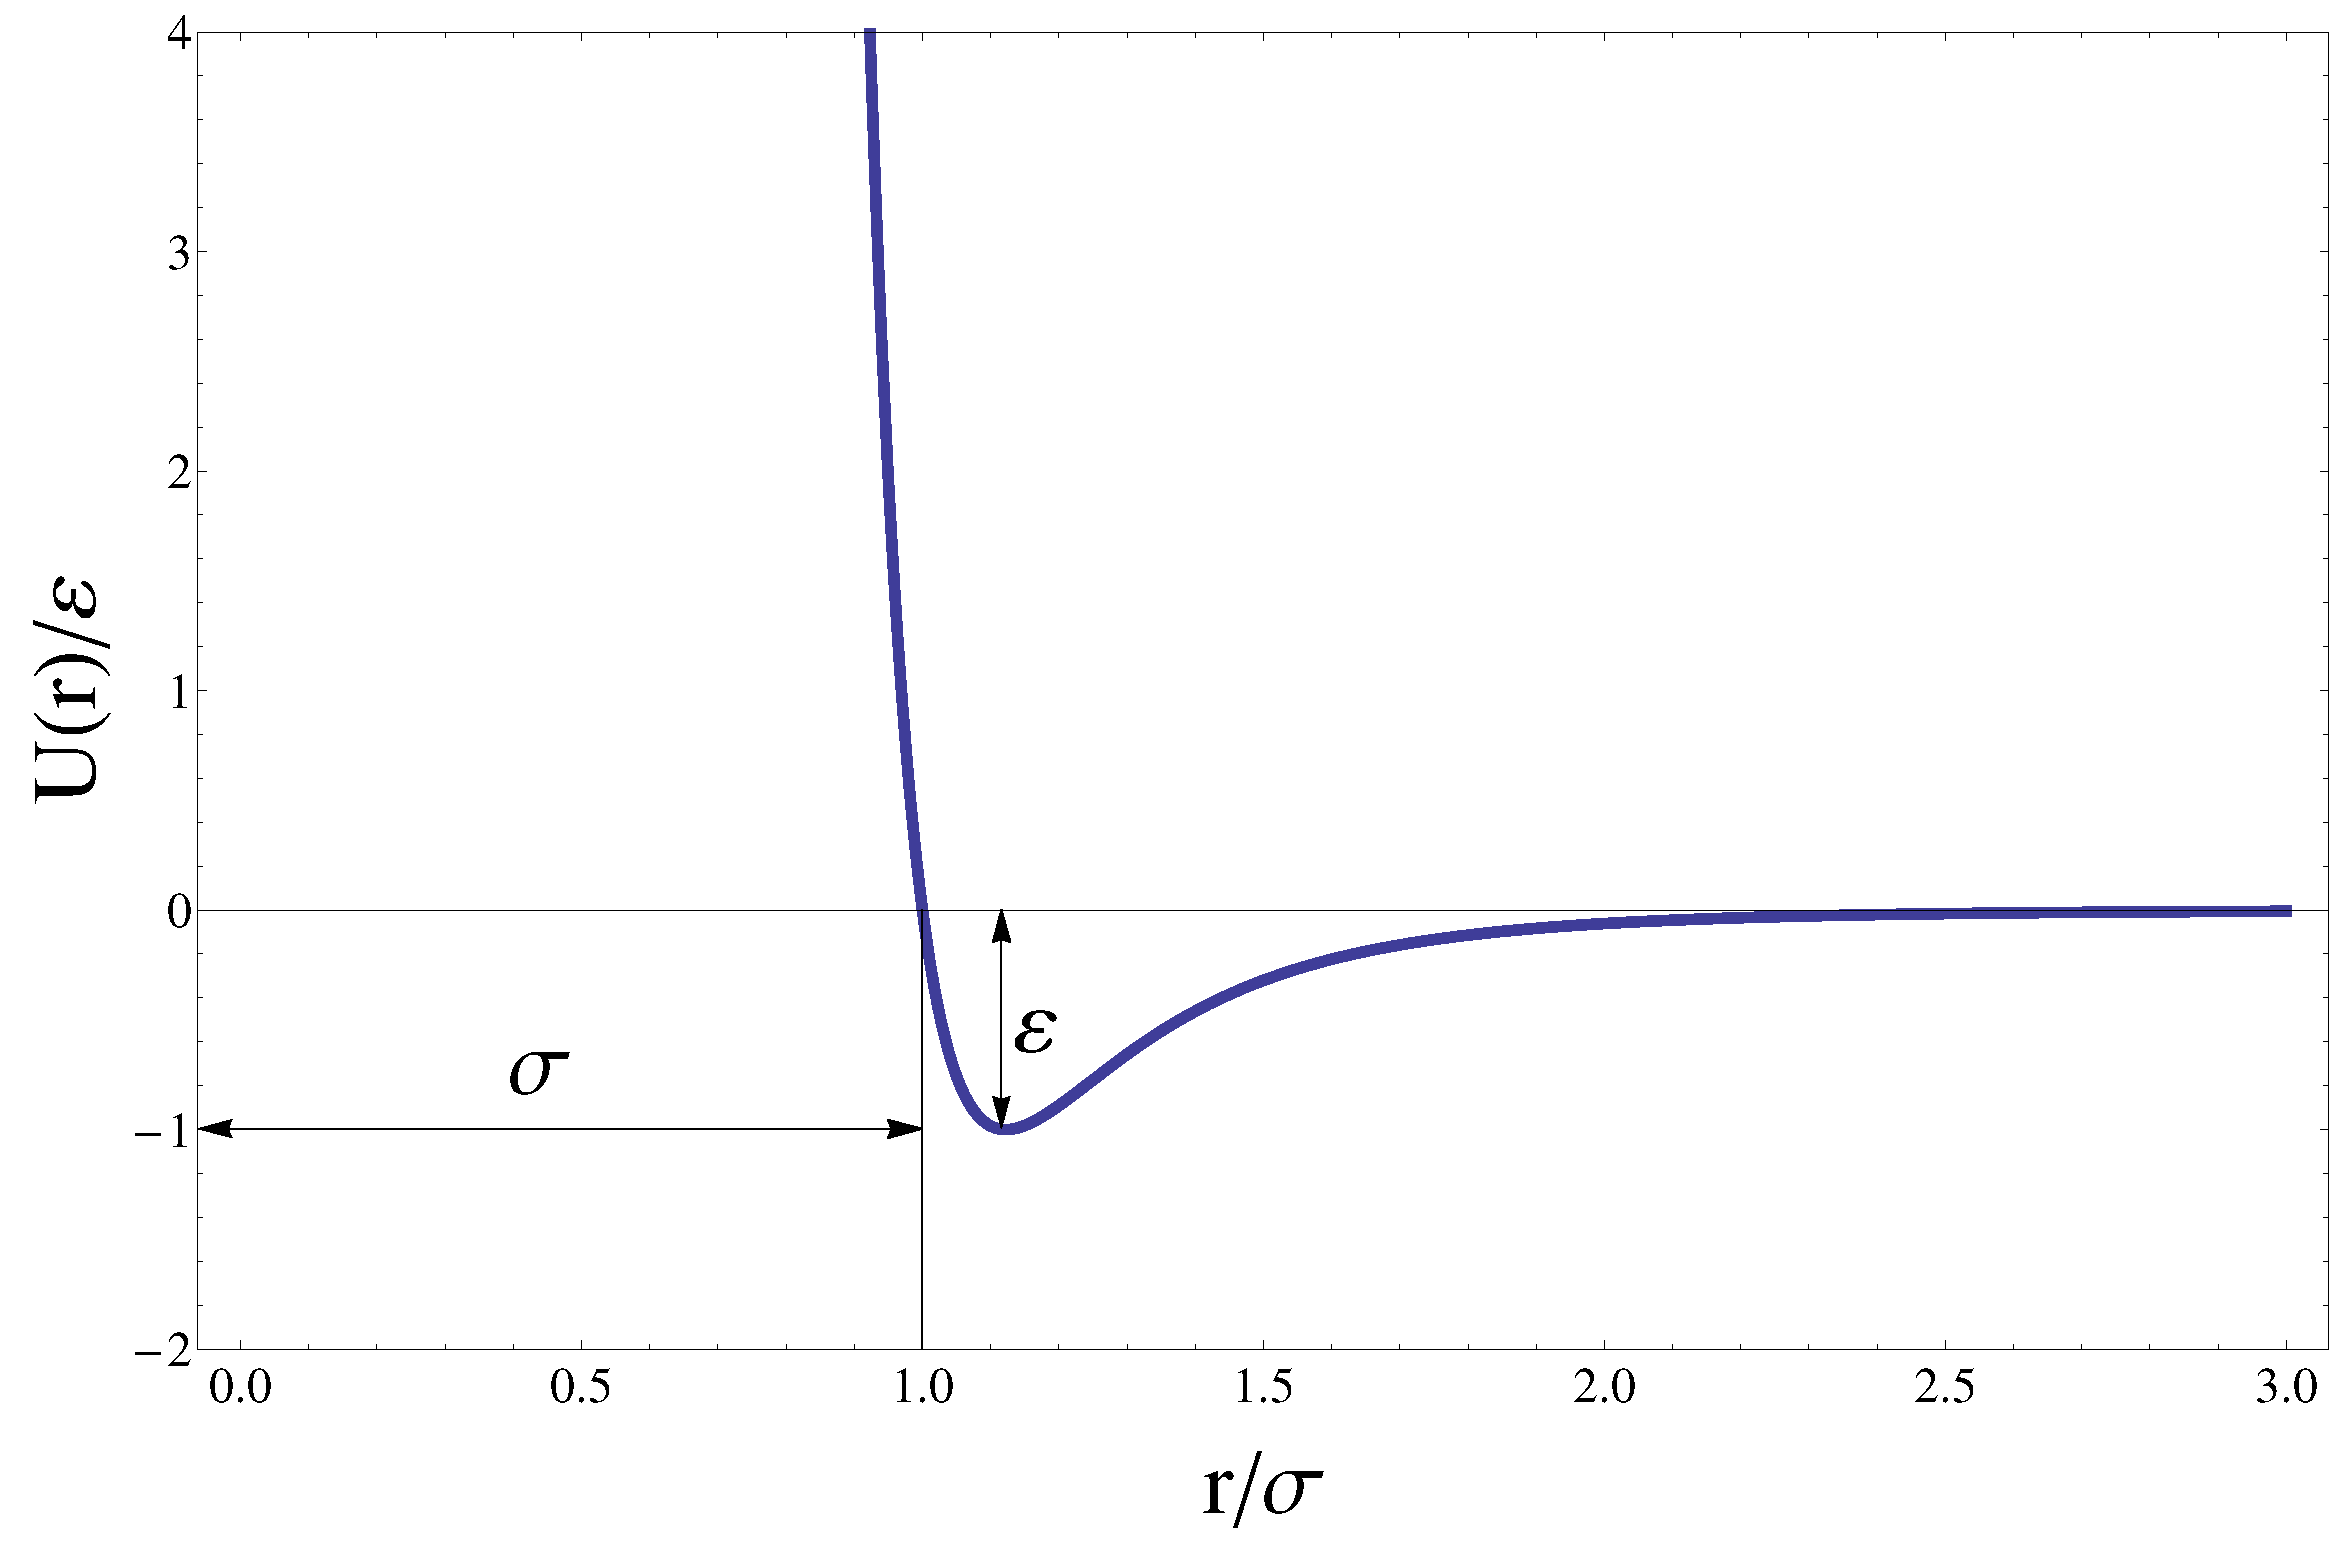
\includegraphics[scale=0.2]{images/LJ-2.pdf}
        \caption{The Lennard-Jones 12-6 potential from \eqref{eq:lj}. The x-axis is the particle distance divided by $\sigma$ and  the y-axis is the
        potential divided by the depth of the potential well.}
        \label{fig:lj}
    \end{center}
\end{figure}
Since $\varepsilon$ and $\sigma$ are crucial parameters for the simulation and do (usually) not change over time, it is practical to use them to
define the dimensions of the system. This means that the unit of distance is $\sigma$, the unit of energy is $\varepsilon$ and the unit of mass is 
the mass of the simulated particle. The so called \textit{reduced units} can be constructed from these three parameters and put into relation to the
original units. Here are some examples:
\begin{itemize}
    \item {distance:} $r^* = r/\sigma$
    \item {potential energy:} $U^* = U/\varepsilon$
    \item {temperature:} $T^* = k_B T/\varepsilon$
    \item {time:} $t^* = t\sqrt{\varepsilon/(m\sigma^2)}$
    \item {pressure:} $P^* = P\sigma^3/\varepsilon$
    \item {density:} $\rho^* = \rho \sigma^3$
\end{itemize}
One very popular choice for the simulated atoms is Argon because it is an inert gas and the atoms behave 
approximately like hard spheres which attract each other with weak van der Waals forces, which justifies the use of the Lennard-Jones potential. 
Argon has a mass of m = $6.69 \times 10^{-26}$ kg, $\sigma = 3.4 \times 10^{-10}$m and $\varepsilon = 1.65 \times 10^{-21}$J.\\
With the above introduced reduced units, the Lennard-Jones potential can be written as
\begin{equation}
    U(r^*) = 4\left[{r^*}^{-12} - {r^*}^{-6}\right].
\end{equation}
Since the reduced units will be used throughout the rest of this thesis, i will drop the asterisk henceforth.\\
From the Lennard-Jones potential the corresponding force can be calculated by taking the derivative with respect to the direction of interest:
\begin{eqnarray}
    F_{x} &=& -\frac{\partial}{\partial x} U(r) \nonumber\\
                &=& -\frac{\partial}{\partial x} 4\left[{r}^{-12} - {r}^{-6}\right] \nonumber\\
                &=& -4 \left[(-12){r}^{-13} - (-6){r}^{-7}\right] \frac{\partial r}{\partial x} \nonumber\\
                &=& 48 \left[r^{-13} - 0.5 \ r^{-7}\right] \frac{x}{r} \nonumber\\
    \label{eq:ljforce} &=& 48 \left[r^{-14} - 0.5 \ r^{-8}\right] x
\end{eqnarray}
The force in the y and z direction can be calculated analogously.\\




%\subsection{The Glass Nanoparticle}
%The glass particle from the experiment will be represented by a system of 864 particles, aligned regularly on a FCC (face centered cubic) lattice.
%This alignment is achieved by defining a minimum cell, containing points:
%\begin{eqnarray*}
    %p_1 &=& \{0,0,0\}\\
    %p_2 &=& \{0.5,0.5,0\}\\
    %p_3 &=& \{0.5,0,0.5\}\\
    %p_4 &=& \{0,0.5,0.5\}
%\end{eqnarray*}
%The whole system is then  created by copying this unit cell.\\
%The interaction between the atoms is modeled by the Lennard-Jones potential. It has the form
%\begin{equation}
    %U(r) = 4\varepsilon\left[\left(\frac\sigma r\right)^{12} - \left(\frac\sigma r\right)^6\right].
%\end{equation}
%To simplify the equation and computation of the potential and other quantities, like the forces or pressure, it is useful to introduce reduced units.
%In general, reduced units BLABLABLA THINK OF GOOD TEXT HEREJKA\\
%The basic units in a system with Lennard-Jones interaction are length ($\sigma$), energy ($\varepsilon$ or $\varepsilon / k_B$) and mass ($m$). Every 
%quantity can now be written in terms of this units, so they become reduced quantities, denotet by an asterisk. The most important ones are:
%\begin{eqnarray*}
    %r^* &=& r/\sigma\\
    %T^* &=& k_B/\varepsilon \ T\\
    %U^* &=& U/\varepsilon \\
    %P^* &=& P \sigma^3/\varepsilon 
%\end{eqnarray*}
%With the above introduced reduced units, the Lennard-Jones potential can be written as
%\begin{equation}
    %U(r^*) = 4\left[{r^*}^{-12} - {r^*}^{-6}\right].
%\end{equation}
%Since this is the most practical form, it will be used without the asterisk from here on.\\
%The Lennard-Jones potential is an additive pair-potential, so the total energy of the system can be calculated by summing over all pairs of atoms:
%\begin{equation}
    %U_{\text{tot}} = \sum_{i=1}^{N-1}\sum_{j=i+1}^N4\left[{r_{ij}}^{-12} - {r_{ij}}^{-6}\right]
%\end{equation}
%where $r_{ij}$ denotes the distance between atom $i$ and $j$. \\
%The Velocity-Verlet algorithm uses the forces to calculate the positions and velocities for the next timestep, we need to calculate the derivative of
%the potential energy:
%\begin{eqnarray}
    %F_{x} &=& -\frac{\partial}{\partial x} U(r) \nonumber\\
                %&=& -\frac{\partial}{\partial x} 4\left[{r}^{-12} - {r}^{-6}\right] \nonumber\\
                %&=& -4 \left[(-12){r}^{-13} - (-6){r}^{-7}\right] \frac{\partial r}{\partial x} \nonumber\\
                %&=& 48 \left[r^{-13} - 0.5 \ r^{-7}\right] \frac{x}{r} \nonumber\\
    %\label{eq:ljforce} &=& 48 \left[r^{-14} - 0.5 \ r^{-8}\right] x
%\end{eqnarray}
%This is the component of the force in x-direction -- the other components are calculated analogously.






\newpage
\section{Results}
% results with different parameters, graphs, etc.





\newpage
\section{Conclusion}
% what does this all tell us? do we need to study more of this? 






\newpage
\bibliography{references}
\bibliographystyle{plain}

\end{document}
